\chapter{A caccia di buchi neri di massa intermedia}
\label{chap:cap1}

In questo Capitolo viene presentato il \textit{background} astrofisico sul quale si sviluppa l'intero lavoro di tesi.\\
Ci si focalizza sull'importanza di voler ricercare i buchi neri di massa intermedia (\textit{Intermediate-Mass Black Holes}, IMBHs) all'interno degli ammassi globulari (\textit{Globular Clusters}, GCs) e vengono presentate alcune tecniche utilizzate per la loro identificazione. In particolare, viene approfondito il metodo di identificazione basato sulla dinamica delle Pulsar Millisecondo (\textit{Millisecond Pulsars, MSPs}) all'interno dei GCs. Infatti, questo progetto si sviluppa in una direzione diversa, ma complementare all'idea suggerita da Abbate el al.(2019) \cite{abbate1:paper} di identificare gli IMBHs nei GCs utilizzando, oltre alle velocità e accelerazioni delle MSPs in ammasso, anche le informazioni dinamiche fornite dalle derivate dell'accelerazione.\\
Nello specifico, nella mia tesi, ho sviluppato un codice che utilizza un modello di \textit{Machine Learning} (ML) interpretabile in grado di fare previsioni sulla presenza di IMBHs in ammassi sulla bese di tali informazioni dinamiche delle MSPs.

\section{I buchi neri di massa intermedia}
\label{sec:IMBH}
I buchi neri vengono classificati in base alla loro massa in: buchi neri di origine stellare, buchi neri di massa intermedia e buchi neri super-massicci.\\
I buchi neri di origine stellare sono oggetti compatti che si formano alla fine della vita di stelle massicce in seguito ad esplosioni di Supernova, mentre i buchi neri super-massicci normalmente si trovano al centro di galassie. I buchi neri di massa intermedia, invece, (\textit{Intermediate-Mass Black Holes}, IMBHs) sono buchi neri la cui massa (tra 100 e $10^{6}$ M$_{\odot}$) è significativamente maggiore di quella dei buchi neri di origine stellare e al contempo molto minore di quella dei buchi neri super-massicci.

I buchi neri sono caratterizzati da intensi campi gravitazionali dai quali, escludendo fenomeni quantistici non ancora verificati sperimentalmente, nulla può fuoriuscire, nemmeno la radiazione. Per questo motivo non possono essere osservati direttamente, ma possiamo unicamente misurare gli effetti che essi hanno sugli altri corpi celesti. Ad esempio, è possibile rilevare le emissioni X quando essi, in un sistema binario, accrescono sottraendo massa ad una stella compagna (Fig.\ref{fig:binario}) o le emissioni sottoforma di onde gravitazionali quando si fondono (fenomeno di \textit{merging}) con altri oggetti compatti o anche si possono rilevare gli effetti gravitazionali che hanno sulle orbite di altri oggetti, come nel caso di un buco nero super-massivo nel centro galattico.
\begin{figure}
\begin{center}
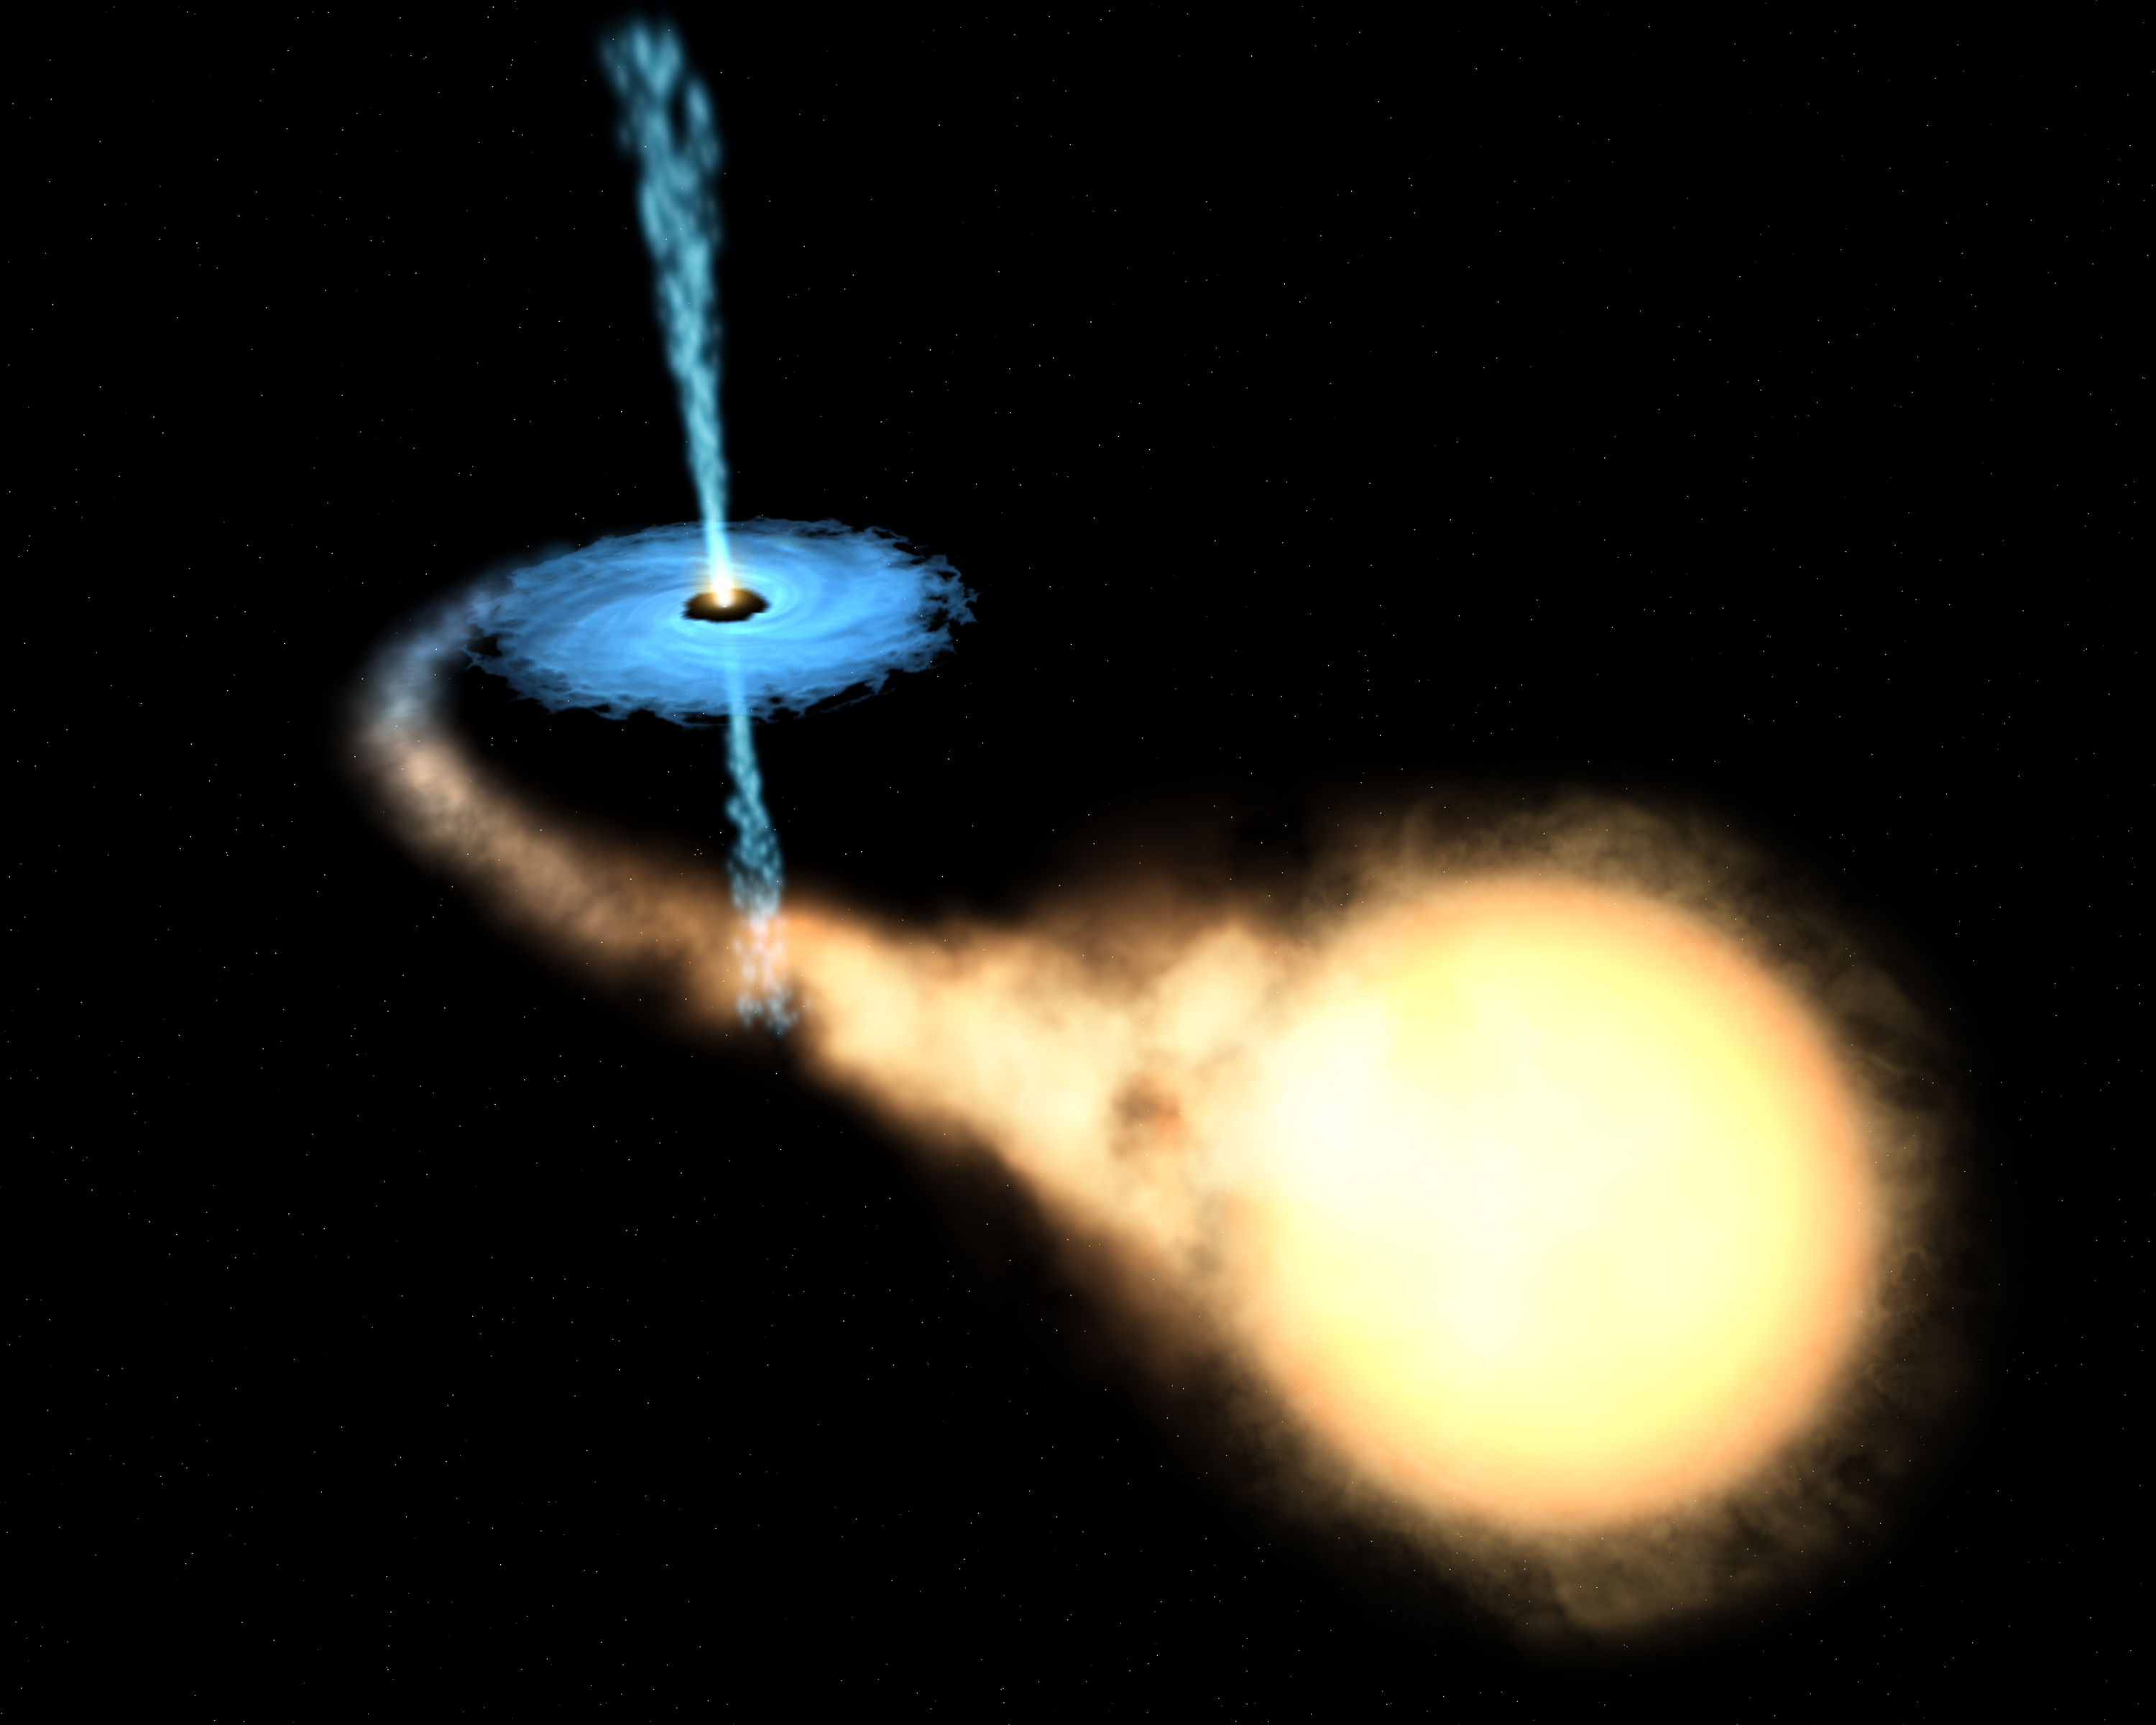
\includegraphics[width=0.4\columnwidth]{images/Accretion_disk.jpg}
\end{center}
\caption{Esempio, in un \textit{artist impression}, di buco nero in un sistema binario che accresce la propria massa a discapito della sua stella compagna \cite{binaria:online}.}
\label{fig:binario}
\end{figure}

Gli IMBHs, oggetto di studio di questa tesi, dal punto di vista osservativo, potrebbero rappresentare il nesso che collega le informazioni raccolte finora e che riguardano principalmente i buchi neri di origine stellare e quelli super-massici. Infatti, nonostante i modelli teorici suggeriscano fortemente che è possibile trovare gli IMBHs all'interno di ammassi globulari \cite{milham:paper}, attualmente non si dispone di prove definitive per confermarlo, in quanto gli indizi che abbiamo sono ancora relativamente controversi e non si è ancora raggiunto il consenso presso la comunità scientifica (Fig.\ref{fig:imbh_gap}).
\begin{figure}[H]
\begin{center}
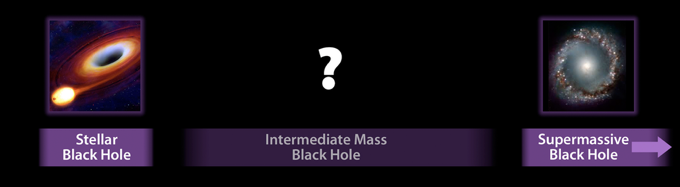
\includegraphics[width=0.7\columnwidth]{images/IMBH_gap.png}
\end{center}
\caption{Vuoto di informazioni tra le categoria di buchi neri di origine stellare ed i buchi neri super-massivi: gli IMBHs.}
\label{fig:imbh_gap}
\end{figure}

Gli scenari di formazione proposti per questi oggetti peculiari sono molteplici \cite{jenny:paper}.\\
Il primo scenario ipotizza che gli IMBHs possono essersi originati in seguito al collasso di stelle di Popolazione III, ovvero ipotetiche stelle formatesi con abbondanza chimica primordiale che possono raggiungere alte masse rispetto alle stelle odierne \cite{abel:paper}.\\
La seconda ipotesi è quella del collasso diretto secondo cui la loro massa si sarebbe addensata direttamente dal materiale dell’universo in formazione subito dopo il \textit{Big Bang}, senza passare per le fasi dell'evoluzione stellare \cite{haehnelt:paper}.\\
Un ultimo interessante scenario, invece, suggerisce che essi si formino mediante fenomeni di collisione e di \textit{merging}. In questo caso esistono più ipotesi.\\ 
Secondo \textit{Miller $\&$ Hamilton 2002} \cite{milham:paper} un buco nero di origine stellare di 50 $M_{\odot}$ potrebbe collocarsi in breve tempo al centro dell’ammasso per l'effetto di segregazione di massa; successivamente, collisioni con altri buchi neri stellari mediate da incontri gravitazionali a tre e quattro corpi e da perdita di energia per emissione di onde gravitazionali, porterebbero al raggiungimento di masse dell’ordine di $10^{3}$ $M_{\odot}$ in un tempo paragonabile a quello di Hubble.\\
Un altro meccanismo, invece, propone che in un $core$ ad alta densità, le stelle molto massicce $\left(50-100 M_{\odot}\right)$ possono essere soggette ad un’efficiente segregazione di massa che le colloca nel nucleo dell’ammasso mentre si trovano in fase di Sequenza Principale. A questo punto si verificherebbe un numero sempre crescente di collisioni e \textit{merging} tra stelle che porterebbero alla formazione e all’immediato collasso di una stella con massa pari a $\simeq 10^{-3}$ volte la massa dell'ammasso, generando così un IMBH \cite{portzw:paper}.\\
I GCs, essendo ambienti stellari densi e dinamicamente attivi, potrebbero essere i luoghi ideali per la formazione di IMBHs attraverso collisioni stellari o incontri gravitazionali tra buchi neri  di origine stellare e successive fusioni \cite{portmcmil:paper}. L'interesse per la formazione di IMBHs in GCs è anche legato al fatto che gli ammassi globulari più massicci tendono a precipitare rapidamente verso il centro della galassia, dove potrebbero concorrere a formare il \textit{nuclear star cluster} \cite{arcasedda:paper}. Pertanto, essi rappresentano un possibile meccanismo di formazione di un buco nero super-massivo attraverso fenomeni di \textit{merging} tra IMBHs.

In condizioni di prossimità ad una binaria di oggetti compatti gli IMBHs possono essere sorgenti di emissione di onde gravitazionali.\\ 
Gli interferometri terrestri di onde gravitazionali LIGO e Virgo \cite{ligo:online}, \cite{virgo:online}, \cite{ligovirgo1:paper} operano in un intervallo di frequenze tra 
qualche decina e qualche migliaio di Hertz. Quindi possono osservare la coalescenza di buchi neri fino ad una massa di
$\sim 500 M_{\odot}$, nel regime degli IMBHs.\\ 
La prossima generazione di interferometri nello
spazio, come il Laser Interferometer Space Antenna, LISA \cite{amaro:paper}, sarà ancora più adatta ad osservare gli IMBHs, poiché opererà nel range di frequenza compreso tra $10^{-3}-10^{-1}$ Hertz.\\
Inoltre, gli IMBHs sono molto difficili da individuare in quanto, gli ammassi globulari sono ambienti decisamente poveri di gas, poiché sono costituiti principalmente da stelle vecchie e il gas primordiale che era presente è stato utilizzato nelle precedenti fasi di formazione stellare o spazzato via da esplosioni di Supernova. Per tale ragione e per come operano i meccanismi di accrescimento, ovvero tramite la dissipazione di energia e momento angolare verso l'esterno di un disco, risulta difficile rilevare emissioni X, determinate da tali fenomeni.\\
Un'altra ragione per cui risulta difficoltoso rilevarli è legata alla componente stellare.\\
Per ogni buco nero di massa $M_{BH}$, infatti, è possibile stimare il raggio di influenza $r_{i}$:
\begin{equation}
r_{i}=\frac{G M_{B H}}{\sigma^{2}}
\label{eq:rinfl}
\end{equation}
con $G$ la costante di gravitazione universale e $\sigma$ la dispersione di velocità delle stelle subito al di fuori della sfera di influenza del buco nero. Le stelle all’interno di questo raggio risentono principalmente dell’influenza gravitazionale del buco nero stesso.\\
Il raggio di influenza di un IMBH è dell'ordine di solo qualche secondo d'arco. Ad esempio, un IMBH di $\sim1000M_{\odot}$ all'interno di \textit{47 Tucanae} avrebbe un raggio di influenza di circa $1"$ \cite{jenny:paper}, contro la dimensione apperente dell'ammasso di circa 31' \cite{47tuc:online}. Pertanto, in generale, la sfera di influenza di un IMBH non è così importante, rispetto alle dimensioni dell'ammasso, da influenzare gravitazionalmente un numero di stelle sufficientemente elevato da determinare una quantità di eventi di accrescimento mareale tale da poter essere osservato. 

\section{Metodi di identificazione di IMBHs al centro di ammassi globulari}
\label{sec:identificazione}

Di fronte alla presenza di un IMBH in un ammasso stellare, ci aspettiamo che si verifichino delle alterazioni nei profili di densità del GC e di dispersione di velocità delle stelle dell'ammasso. Sulla base di questi si costruiscono la maggior parte dei metodi di identificazione degli IMBHs con le relative difficoltà a livello pratico. Inoltre, se ci trovassimo in presenza di un fenomeno di accrescimento, la misurazione delle emissioni X e radio sarebbe un altro canale identificativo di IMBH al centro di un GC \cite{strader:paper}.

Un IMBH aumenta la profondità della buca di potenziale di un ammasso causando un incremento della densità stellare nelle zone centrali. Queste ultime, pertanto, risultano avere un profilo di densità di una \textit{cuspide} ben descritta dalla legge di potenza $\rho \propto r^{-\alpha}$, con $\alpha \simeq 1.55$ \cite{baum:paper}.  

Le stelle all’interno del raggio di influenza $r_{i}$ (eq. \ref{eq:rinfl}) del IMBH, oltre a risentire principalmente dell’influenza gravitazionale del buco nero, seguono un profilo di dispersione di velocità di tipo \textit{kepleriano} caratterizzato da una ripidità nelle regioni centrali. Tuttavia, la determinazione accurata della dispersione di velocità delle stelle valutata solo nella regione centrale del GC, è al limite delle capacità dell’attuale strumentazione astronomica e richiede un’elevatissima risoluzione spaziale. I risultati di misurazioni effettuate con metodi diversi (spettroscopia in luce integrata, stelle individuali, studio dei moti propri) sono talvolta in disaccordo tra loro, con la conseguenza che la comunità scientifica non ha ancora raggiunto un consenso in merito \cite{lutz1:paper}.\\
Il profilo di dispersione di velocità, però si può ottenere teoricamente sulla base del profilo di densità determinato precedentemente e considerando un oggetto puntiforme di una certa massa al centro dell’ammasso \cite{lutz:paper}.\\
Come risultato si ottiene una famiglia di profili di dispersione di velocità che, una volta confrontati con le osservazioni, restituiscono la massa del BH centrale (Fig.\ref{fig:profili_vel}).
\begin{figure}[ht]
\begin{center}
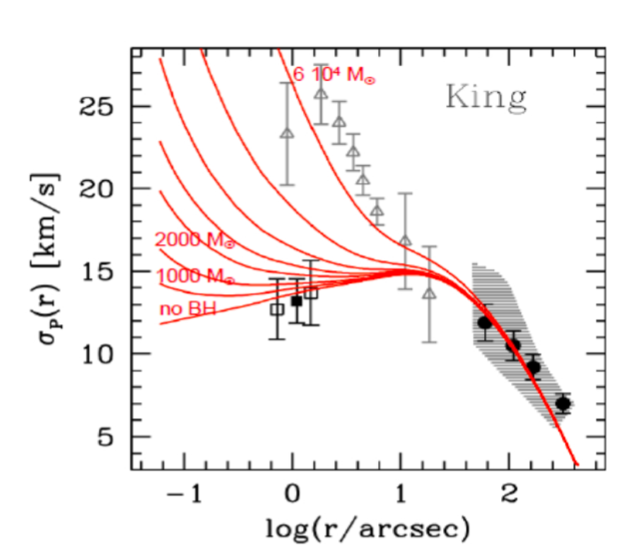
\includegraphics[width=0.6\columnwidth]{images/profili_vel.png}
\end{center}
\caption{Profilo di dispersione di velocità osservato per l'ammasso globulare NGC 6388 con sovrapposte le linee rosse continue delle famiglie di modelli considerate. Esse sono state ottenute assumendo una diversa massa per il buco nero centrale. Si noti che aumentando la massa del IMBH la pendenza nelle regioni centrali risulta più ripida \cite{Lanzoni:paper}, \cite{lutz:paper}.}
\label{fig:profili_vel}
\end{figure}

Tuttavia, la presenza di una \textit{cuspide} nelle regioni centrali di un GC può essere dovuta anche a cause diverse dalla presenza di un IMBH. Ad esempio, a seguito di un collasso del \textit{core}, tanti buchi neri di massa stellare potrebbero trovarsi nelle regioni centrali dell'ammasso e determinare, quindi, i ripidi profili di velocità e densità associati alle cuspidi \cite{trenti:paper}. Questo vuol dire, in altre parole, che la presenza di una cuspide non è sufficiente per affermare che al centro dell'ammasso ci sia un IMBH. Ma anche il viceversa non è sufficiente per affermare il contrario. Infatti, la non rilevazione di una cuspide non esclude a priori la presenza di un IMBH centrale. Come abbiamo già visto, infatti, la sfera di influenza di un IMBH potrebbe rivelarsi decisamente troppo piccola per far sì che la cuspide si veda.

Oltre ai metodi che si servono della dinamica stellare in ammasso e dei moti propri delle stelle \cite{banwolf:paper}, \cite{gebh:paper}, un altro metodo per l'dentificazione degli IMBH potrebbe essere quello che si basa sul rilevamento dell'emissione X e radio degli IMBHs in fase di accrescimento \cite{mac1:paper}, \cite{mac2:paper}.\\
Tali emissioni, però, risultano difficili da osservare nei GCs poichè si tratta di sistemi poveri di gas. Tuttavia, recentemente, le prove dell'esistenza di un IMBH in un GC potrebbero essere fornite dall'osservazione di un evento di disturbo di marea in un ammasso extra-galattico \cite{lin:paper}. I dati in X sono stati raccolti dai telescopi in orbita \textit{Chandra} e \textit{XMM-Newton} e successivamente confermati dal \textit{Telescopio Spaziale Hubble}. Attualmente si stanno svolgendo ulteriori indagini osservative per identificare la natura dell'oggetto responsabile dell'evento, ma gli autori dello studio, \textit{Lin D. et al. 2020} \cite{lin_2020:paper}, sostengono si tratti di un IMBH in procinto di inglobare una stella.\\
\indent
Oltre a questi, esistono anche metodi indiretti per rilevare IMBH al centro di ammassi. Uno tra questi è quello che si basa sull'effetto degli IMBHs sulla segregazione di massa \cite{pasquato:paper}. Nei GCs, ci si aspetta, infatti, che gli IMBHs per la maggior parte del tempo si trovino in sistemi binari con altri oggetti massicci, come buchi neri di origine stellare. In questa configurazione essi inietterebbero energia nel nucleo del GC, attenuando la segregazione di massa stellare. Anche le binarie primordiali, però, potrebbero essere responsabili dello stesso fenomeno. Ciò porterebbe ad un problema di degenerazione nell'indicatore di segregazione di massa, che potrebbe essere risolto misurando la frazione di binarie nel \textit{core} in maniera indipendente. Questo, però, ha le sue complicazioni dovute ai problemi di risoluzione spaziale di cui si è già parlato. Anche per questo motivo gli studi portati avanti sulla base di tale metodologia non sono ancora stati in grado di rilevare forti candidati di GCs che ospiterebbero un IMBH.

Tutti i metodi presentati riscontrano delle difficoltà nell'identificazione degli IMBHs all'interno degli ammassi. Queste sono legate soprattuto ai fattori che ne influenzano la rilevazione diretta. Gli IMBHs, infatti, risultano così sfuggenti principalmente a causa dei problemi che comporta la piccola dimensione della loro sfera di influenza e, conseguentemente, dei problemi osservativi relativi alla risoluzione spaziale per i \textit{core} degli ammassi.
Per tali ragioni risulta interessante approfondire un metodo alternativo e indiretto per la ricerca di IMBHs all'interno di ammassi globulari: quello che si basa sullo studio delle proprietà dinamiche delle Pulsar Millisecondo (\textit{Millisecond Pulsars, MSPs}) \cite{pere:paper}, \cite{abbate:paper}.  
I paragrafi successivi, infatti, saranno dedicati all'approfondimento di tale metodo che è proprio quello su cui si basa questo progetto di tesi.

\section{Metodo delle MSPs}
\label{sec:MSP}

Le MSPs sono oggetti molto frequenti nei GCs ed essendo caratterizzate da periodi di rotazione estremamente stabili, possono essere utilizzate come strumento per l'identificazione di IMBHs all'interno di ammassi globulari. Infatti, le misure ottenute per effetto Doppler permettono di avere informazioni sulle loro accelerazioni e sulle derivate temporali di ordine superiore.\\
In particolare, le derivate prima, detta \textit{jerk}, e seconda, detta \textit{jounce} o \textit{snap}, dell'accelerazione delle MSPs in ammassi, sono state valutate in maniera più approfondita nel recente articolo di Abbate et al. (2019) \cite{abbate1:paper}.\\
\MP{Pero l'articolo di Abbate e puramente simulativo; andrebbe scovata una referenza osservativa su che cosa si puo veramente misurare sulle pulsar reali}
\subsection{Profili radiali di Jerk e Snap in ammasso}
\label{subsec:profili}

Analiticamente è possibile derivare le relazioni matematiche che descrivono i profili radiali di \textit{jerk} e \textit{snap} di stelle in ammasso \cite{abbate1:paper}.

Consideriamo una stella di prova che sperimenta l'attrazione gravitazionale del campo generato da tutte le stelle dell'ammasso, in particolare assumiamo che il GC sia descritto dal profilo di King \cite{king:paper}.\\
L'accelerazione in funzione della distanza \textit{r} dal centro dell'ammasso, nelle regioni centrali del GC, può essere approssimata come:
\begin{equation}
   \textbf{a}(r) = -4 \pi G \rho_{c} r_{c}^{3} \left[\sinh^{-1} \left(\frac{r}{r_{c}}\right) - \frac{r}{r_{c}\sqrt{1+({r}/{r_c})^{2}}}\right] \frac{\textbf{r}}{r^{3}} = -\left | a \right | \frac{\textbf{r}}{r}
   \label{eq:accrad_king}
\end{equation}
dove $\rho_{c}$ è la densità centrale dell'ammasso ed $r_{c}$ il raggio del $core$.\\
Per calcolare il $jerk$ è necessario derivare rispetto al tempo l'equazione \ref{eq:accrad_king}, ottenendo:
\begin{equation}
\mathbf{\Dot{a}}_{K}(r)=-\frac{d|a(r)|}{d t} \frac{\mathbf{r}}{r}-|a(r)| \frac{\mathbf{v}}{r}+|a(r)| \frac{(\mathbf{v} \cdot \mathbf{r}) \mathbf{r}}{r^{3}}
\label{eq:jerk_king}
\end{equation}
in cui la derivata temporale della norma dell'accelerazione è data da:
\begin{equation}
\frac{d|a(r)|}{d t}=-2 \frac{v|a(r)|}{r}+4 \pi G v \rho_{\mathrm{c}}\left(\frac{1}{1+\left(r / r_{\mathrm{c}}\right)^{2}}\right)^{\frac{3}{2}}
\end{equation}
con $v$ la norma della velocità.\\
Nel caso in cui il GC fosse caratterizzato da forti fenomeni di collisioni stellari, anche i $jerk$ potrebbero risultare influenzati dalle stelle vicine. In questo caso, il $jerk$ sarebbe caratterizzato dalla seguente distribuzione di probabilità \cite{prager:paper}:
\begin{equation}
P(\dot{a})=\frac{1}{\pi^{2}} \frac{\dot{a}_{0}}{\left(\dot{a}^{2}+\dot{a}_{0}^{2}\right)^{2}}
\end{equation}
in cui $\dot{a}_{0}$ è il $jerk$ caratteristico dato da:
\begin{equation}
\dot{a}_{0}=\frac{2 \pi \xi}{3} G\langle m\rangle \sigma n
\end{equation}
dove $\xi$=3.04 è una costante numerica, $\langle m \rangle$ è la massa media delle stelle, $\sigma$ è la dispersione di velocità ed $n$ è la densità numerica delle stelle.\\
La distribuzione dei $jerk$ proiettata lungo la linea di vista $\dot{a}_{l}$ è una distribuzione Lorentziana:
\begin{equation}
P\left(\dot{a}_{l}\right)=\frac{1}{\pi} \frac{\dot{a}_{0}}{\dot{a}_{l}^{2}+\dot{a}_{0}^{2}}
\end{equation}
Se all'interno del GC vi è un IMBH, il $jerk$ della stella di prova sarà influenzato dalla massa centrale $M$ ed il profilo sarà:
\begin{equation}
\dot{\mathbf{a}}_{M}=-G M\left(\frac{\mathbf{v}}{r^{3}}-3 \frac{(\mathbf{v} \cdot \mathbf{r}) \mathbf{r}}{r^{5}}\right)
\label{eq:jerk_imbh}
\end{equation}
dove \textbf{r} è la distanza dalla massa $M$ e \textbf{v} è la relativa velocità.\\
Inoltre l'IMBH crea una sovra-densità stellare caratterizzata da un profilo radiale con \textit{slope} pari a -1.55 \cite{baum:paper}:
\begin{equation}
\dot{\mathbf{a}}_{\mathrm{cusp}}=\left\{\begin{array}{l}
-\frac{4 \pi G}{1.45} r_{\mathrm{i}}^{1.55} \rho_{\mathrm{i}}\left(\frac{\mathrm{v}}{r^{1.55}}-1.55 \frac{(\mathrm{v} \cdot \mathrm{r}) \mathrm{r}}{r^{3.55}}\right) \text { for } r<r_{\mathrm{i}} \\
-\frac{4 \pi G}{1.45} r_{\mathrm{i}}^{3} \rho_{\mathrm{i}}\left(\frac{\mathrm{v}}{r^{3}}-3 \frac{(\mathrm{v} \cdot \mathrm{r}) \mathrm{r}}{r^{5}}\right) \text { for } r>r_{\mathrm{i}}
\end{array}\right.
\label{eq:jerk_cusp}
\end{equation}
in cui $r_{i}$ è il raggio di influenza dell'IMBH e $\rho_i$ è il valore di densità a tale raggio.

Derivando rispetto al tempo le equazioni \ref{eq:jerk_king}, \ref{eq:jerk_imbh} e \ref{eq:jerk_cusp} è possibile ottenere anche i profili radiali degli $snap$ all'interno degli ammassi.\\
Il contributo del campo gravitazionale dell'intero ammasso è dato dalla:
\begin{equation}
\begin{aligned}
\ddot{\mathbf{a}}_{K}&=-\frac{d^{2}|a(r)|}{d t^{2}} \frac{\mathbf{r}}{r}-2 \frac{d|a(r)|}{d t} \frac{\mathbf{v}}{r}+2 \frac{d|a(r)|}{d t} \frac{(\mathbf{v} \cdot \mathbf{r}) \mathbf{r}}{r^{3}}+\\
&+5|a(r)| \frac{(\mathbf{v} \cdot \mathbf{r}) \mathbf{v}}{r^{3}}-3|a(r)| \frac{(\mathbf{v} \cdot \mathbf{r})^{2} \mathbf{r}}{r^{5}}
\end{aligned}
\label{eq:snap_king}
\end{equation}
Analogamente a quanto calcolato per i $jerk$, anche per gli $snap$ la presenza di un IMBH al centro dell'ammasso porta a due contributi.\\
Il contributo che dipende direttamente dalla massa centrale $M$:
\begin{equation}
\ddot{\mathbf{a}}_{M}=G M\left(-2 a \frac{\mathbf{r}}{r^{4}}-6 \frac{(\mathbf{v} \cdot \mathbf{r}) \mathbf{v}}{r^{5}}-3 \frac{v^{2} \mathbf{r}}{r^{5}}+15 \frac{(\mathbf{v} \cdot \mathbf{r})^{2} \mathbf{r}}{r^{7}}\right)
\label{eq:snap_imbh}
\end{equation}
ed il contributo che determina una sovra-densità. Per quest'ultimo distinguiamo due casi.\\ 
Per $r<r_{i}$:
\begin{equation}
\begin{array}{r}
\ddot{\mathbf{a}}_{\text {cusp }}=-\frac{4 \pi G}{1.45} r_{1}^{1.55} \rho_{i} \left(-0.45 \frac{a \mathbf{r}}{r^{2.55}}-3.1 \frac{(\mathbf{v} \cdot \mathbf{r}) \mathbf{v}}{r^{3.55}}-\right.\\
\left.-1.55 \frac{v^{2} \mathbf{r}}{r^{3.55}}+5.5 \frac{(\mathbf{v} \cdot \mathbf{r})^{2} \mathbf{r}}{r^{5.55}}\right)
\end{array}
\label{eq:snap_cusp1}
\end{equation}
e per $r>r_{i}$:
\begin{equation}
\begin{array}{r}
\ddot{\mathbf{a}}_{\mathrm{cusp}}=-\frac{4 \pi G}{1.45} r_{\mathrm{i}}^{3} \rho_{\mathrm{i}}\left(-2 \frac{a \mathbf{r}}{r^{4}}-6 \frac{(\mathbf{v} \cdot \mathbf{r}) \mathbf{v}}{r^{5}}-5 \frac{v^{2} \mathbf{r}}{r^{5}}+\right. \\
\left.+15 \frac{(\mathbf{v} \cdot \mathbf{r})^{2} \mathbf{r}}{r^{7}}\right)
\end{array}
\end{equation}

\subsection{Metodo osservativo}
\label{subsec:pulsar_timing}

Un ammasso globulare normalmente è caratterizzato in media da un numero di pulsar molto basso, solo in alcuni casi si raggiunge l'ordine di qualche decina di pulsar \cite{pulsar:online}. Esse si localizzano nelle regioni più interne degli ammassi e di solito circa la metà si trova in sistemi binari.

Dal punto di vista pratico, per identificare IMBHs all'interno di GCs basterebbero le informazioni fornite dalle accelerazioni se avessimo a disposizione un numero consistente di pulsar per ogni ammasso. Ma per ovviare al problema delle poche pulsar normalmente presenti in questi sistemi, si potrebbero estrarre più informazioni da ognuna di esse considerando anche \textit{jerk} e \textit{snap}. Per mezzo delle osservazioni, queste quantità si potrebbero ottenere proprio grazie ai periodi prolungati delle MSPs nei GCs.\\
Infatti, le misure delle derivate seconda e terza del periodo di rotazione di un insieme di MSPs in un GC galattico sono fondamentali perché correlano con la componente lungo la linea di vista di \textit{jerk} e \textit{snap}.\\
I tempi di osservazione richiesti per ottenere tali informazioni e per raggiungere una precisione adeguata sono molto lunghi, dell'ordine di diversi anni. Gli autori, però, ritengono che portando avanti queste campagne osservative in maniera regolare, le MSPs potrebbero diventare un buon strumento per l'identificazione di IMBHs al centro degli ammassi.

La derivata prima del periodo è principalmente influenzata dalla componente dell'accelerazione misurata lungo la linea di vista, mentre le derivate seconda e terza del periodo dipendono in maniera diretta da \textit{jerk} e \textit{snap} rispettivamente.\\
La relazione tra accelerazione lungo la linea di vista $a_{c}$ e derivata del periodo $\dot{P}$ della MSPs è data da:
\begin{equation}
\left(\frac{\dot{P}}{P}\right)_{\text {meas }}=\left(\frac{\dot{P}}{P}\right)_{\text {int }}+\frac{a_{\mathrm{c}}}{c}+\frac{a_{\mathrm{g}}}{c}+\frac{\mu^{2} D}{c}
\label{eq:ac_ppunto}
\end{equation}
in cui $(\dot{P} / P)_{\text {int }}$ è la componente intrinseca dovuta allo \textit{spin-down} della pulsar, $a_{g}$ è l'accelerazione dovuta al potenziale galattico lungo la linea di vista e l'ultimo addendo rappresenta l'effetto Shklovskii \cite{shklov:paper}, in cui $\mu$ è il moto proprio della pulsar, $D$ è la distanza dell'ammasso dal Sole e $c$ è la velocità della luce.\\
Gli ultimi due termini generalmente possono essere trascurati rispetto al contributo dato dal termine $a_{c}$ \cite{abbate:paper}. Purtroppo, però, è molto difficile distinguere gli effetti dell'accelerazione dell'ammasso dallo \textit{spin-down} intrinseco. Qualsiasi lavoro focalizzato sulla misurazione dell'accelerazione in un GC a partire da $\dot{P}$, avrà grandi incertezze dovute all'ignoto \textit{spin-down} intrinseco.\\
Tuttavia, in maniera indipendente è possibile stimare l'accelerazione delle MSPs in ammasso solo se esse appartengono ad un sistema binario utilizzando l'effetto Doppler.

Per quanto riguarda \textit{jerk} e \textit{snap} la situazione cambia.\\ 
Le relazioni che legano le derivate seconda e terza del periodo a \textit{jerk}, $\dot{a_{c}}$, e \textit{snap}, $\ddot{a_{c}}$, rispettivamente sono date da:
\begin{equation}
\left(\frac{\ddot{P}}{P}\right)_{\text {meas }}=\frac{\ddot{\mathrm{a}}_{\mathrm{c}}}{c}+\left(\frac{\ddot{P}}{P}\right)_{\text {int }}
\label{eq:jerk_p}
\end{equation}

\begin{equation}
\left(\frac{\dddot{P}}{P}\right)_{\text {meas }}=\frac{\ddot{\mathrm{a}}_{\mathrm{c}}}{c}+\left(\frac{\dddot{P}}{P}\right)_{\text {int }}
\label{eq:snap_p}
\end{equation}
In questi casi i termini di \textit{spin-down} sono praticamente trascurabili (per ulteriori chiarimenti si rimanda il lettore a \cite{abbate1:paper}). Questo vuol dire che misure di derivata seconda e terza del periodo corrispondono direttamente a misure di \textit{jerk} e \textit{snap}.

\subsection{Simulazioni e sviluppi con modelli di\\ Machine Learning}
\label{subsec:sim_ml}

Abbate et al. (2019) \cite{abbate1:paper} sviluppano un set di simulazioni a N-corpi di ammassi stellari in cui calcolano \textit{jerk} e \textit{snap} in maniera auto-conistente, trattando le MSPs come particelle di prova.

In primo luogo, dimostrano che la presenza di un IMBH influenza l'andamento di \textit{jerk} e \textit{snap} in funzione della distanza dal centro del GC, specialmente nelle regioni centrali dell'ammasso (Fig. \ref{fig:profili}).

Successivamente, a seguito di un'analisi condotta utilizzando la statistica Bayesiana, gli autori mostrano che con le derivate delle accelerazioni, in particolare con i \textit{jerk}, per identificare un IMBH di massa dell'ordine di $10^{2}M_{\odot}$ è necessario avere a disposizione un numero di MSPs pari a circa 40, di cui 20 devono trovarsi in sistemi binari. 

Sulla base di tale lavoro, nasce poi l'idea nuova e sviluppata in questa tesi di prevedere la presenza degli IMBHs all'interno dei GCs tramite un modello di ML. I dati utilizzati nella tesi sono stati ottenuti dalle simulazioni di ammassi globulari condotte dagli autori.    
\begin{figure}
\begin{center}
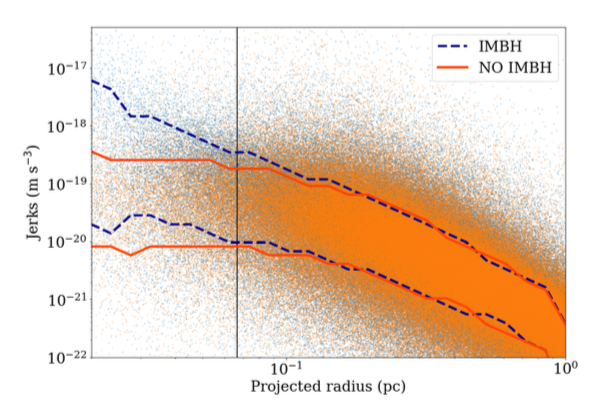
\includegraphics[width=0.6\columnwidth]{images/jerk_rad.png}
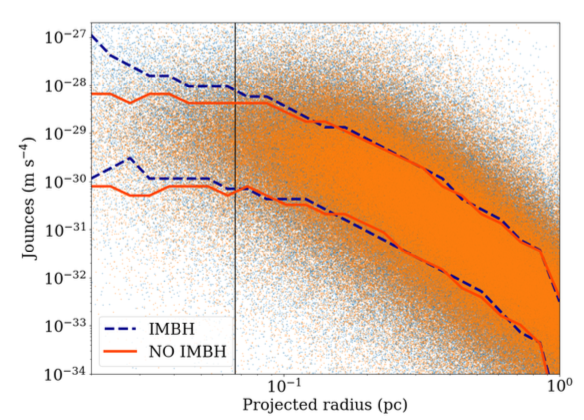
\includegraphics[width=0.6\columnwidth]{images/snap_rad.png}
\end{center}
\caption{Profili radiali di $jerk$ (in alto) e $snap$ (in basso) ottenuti dalle simulazioni di Abbate et al.2019.}
\label{fig:profili}
\end{figure}
